% /solutions/conference-talks/conference-ornate-20min.fr.tex, 22/02/2006 De Sousa
\documentclass{beamer}
\usepackage{listings}
\usepackage{mdframed}
\usepackage{tikz}
\usepackage[overlay,absolute]{textpos}
\usepackage{bbding}
\usepackage{pifont}% http://ctan.org/pkg/pifont
% Ce fichier est un exemple d'expos\'e

% - pour des conf\'erences,
% - d'une dur\'ee approximative de 20 minutes,
% - avec un style ornemental.


% Copyright 2004 by Till Tantau <tantau@users.sourceforge.net>.
%
% Traduction de Philippe De Sousa <philippejjg@free.fr>
%
% En principe, ce fichier peut être redistribu\'e et/ou modifi\'e conform\'ement
% aux termes de la GNU Public License, version 2.
%
% Cependant, ce fichier est suppos\'e comme \'etant un "exemple-type" qui peut être modifi\'e
% selon vos propres besoins. Pour cette raison, si vous utilisez ce fichier en tant qu'
% "exemple-type" et non sp\'ecifiquement pour le distribuer en tant que partie d'un
% package ou programme, je vous donne la permission exceptionnelle de copier librement et
% de modifier ce fichier et même d'effacer ce message de copyright.
\usepackage{pdfpages}

\usepackage[francais]{babel}
% or autre comme par exemple \usepackage[english]{babel}

\usepackage[utf8]{inputenc}
% or autre

\usepackage{float}
\usepackage{graphicx}
\usepackage{wrapfig}
\usepackage{times}
\usepackage[T1]{fontenc}
\makeatletter
\hypersetup{pdfpagemode=FullScreen}
\definecolor{darkblue}{RGB}{57,80,111}

\newcommand{\firstlogo}{images/logos/FACT_official.png}
\newcommand{\secondlogo}{images/logos/ups.jpg}
\newcommand{\footsubject}{Quels sont les systèmes à mettre en œuvre pour offrir une expérience sociale depuis sa télévision ?} % Subject in footer
\newcommand{\xmark}{\ding{55}}%
\newcommand{\cmark}{\ding{51}}%

\newcommand{\rgbcolortheme}{75,106,149}

\mode<presentation> {
\usepackage{../beamer-theme/beamerthemeUNLTheme}
}

\title[] % (facultatif, \`a utiliser uniquement si le titre de l'article est trop long)
{La télévision sociale}
\subtitle{Travail Encadré de Recherche}

\newcommand{\authors}{%
Antoine de \bsc{Roquemaurel}\newline Florent \bsc{Berbie}\newline Cédric \bsc{Rohaut}\newline Manantsoa Andriamihary \bsc{Razanajatovo}
}
\newcommand{\FlorentSpeak}{%
\author[
\textbf{\color{white} F}lorent\\
\textbf{A}ntoine\\
\textbf{C}édric\\
Manan\textbf{T}soa
]{\authors}
}

\newcommand{\AntoineSpeak}{%
\author[
\textbf{F}lorent\\
\textbf{\color{white} A}ntoine\\
\textbf{C}édric\\
Manan\textbf{T}soa
]{\authors}
}

\newcommand{\CedricSpeak}{%
\author[
\textbf{F}lorent\\
\textbf{A}ntoine\\
\textbf{\color{white}C}édric\\
Manan\textbf{T}soa
]{\authors}
}

\newcommand{\TsooSpeak}{
\author[
\textbf{F}lorent\\
\textbf{A}ntoine\\
\textbf{C}édric\\
Manan\textbf{\color{white}T}soa
]{\authors}
}

\newcommand{\NooneSpeak}{
\author[
\textbf{F}lorent\\
\textbf{A}ntoine\\
\textbf{C}édric\\
Manan\textbf{T}soa
]{\authors}
}
\author[
\textbf{F}lorent\\
\textbf{A}ntoine\\
\textbf{C}édric\\
Manan\textbf{T}soa
] % (facultatif, \`a utiliser seulement avec plusieurs auteurs)
{\authors}

\institute[] % (facultatif mais g\'en\'eralement n\'ecessaire)
{
  Universit\'e Toulouse III -- Paul Sabatier \\
  M1 Informatique -- Développement Logiciel 
  \vspace{-10px}
}

\date[ ~ ~ ~ 03 / 04 / 2015] % (facultatif, peut être une abr\'eviation du nom de la conf\'erence)
{Vendredi 03 Avril 2015}

\subject{~}

 \pgfdeclareimage[width=2.5cm]{le-logo}{images/logos/FACT_official.png}
 \logo{\pgfuseimage{le-logo}}


% \`a supprimer si vous ne voulez pas que la table des mati\`eres apparaisse
% au d\'ebut de chaque sous-section : 
\AtBeginSection[] {
  \begin{frame}<beamer>{Ligne directrice}
    \tableofcontents[currentsection]
  \end{frame}
}
% Si vous souhaitez recouvrir vos transparents un \`a un,
% utilisez la commande suivante (pour plus d'info, voir la page 74 du manuel
% d'utilisation de Beamer (version 3.06) par Till Tantau) :

%\beamerdefaultoverlayspecification{<+->}
\newcommand{\happyUser}{%
			\begin{textblock}{5}(14,1.8)
				
\includegraphics[width=1.0cm]{user_happy.png}\\
				\tiny Utilisateur
			\end{textblock}
}

\newcommand{\unhappyUser}{%
			\begin{textblock}{5}(14,1.8)
				
\includegraphics[width=1.0cm]{user_unhappy.png}\\
				\tiny Utilisateur
			\end{textblock}
}
\newcommand{\happyAndUnhappyUser}{%
			\begin{textblock}{5}(13,1.8)
				
\includegraphics[width=1.0cm]{user_unhappy.png}
				
\includegraphics[width=1.0cm]{user_happy.png}\\
				\hspace{10px}
				\tiny Utilisateur
			\end{textblock}
}


\begin{document}
	\sidetoc{no}
	\begin{frame}
		\titlepage
	\end{frame} 
	
	\AntoineSpeak{}
	\begin{frame}{Introduction} \begin{itemize}
		\item Les objets sont de plus en plus connectés\\
			$\Rightarrow$ Internet des objets
		\pause
		\vfill
		\item La télévision est limitée sur le plan social
	\end{itemize}
		\vfill
			\begin{figure}[H]
				\centering
				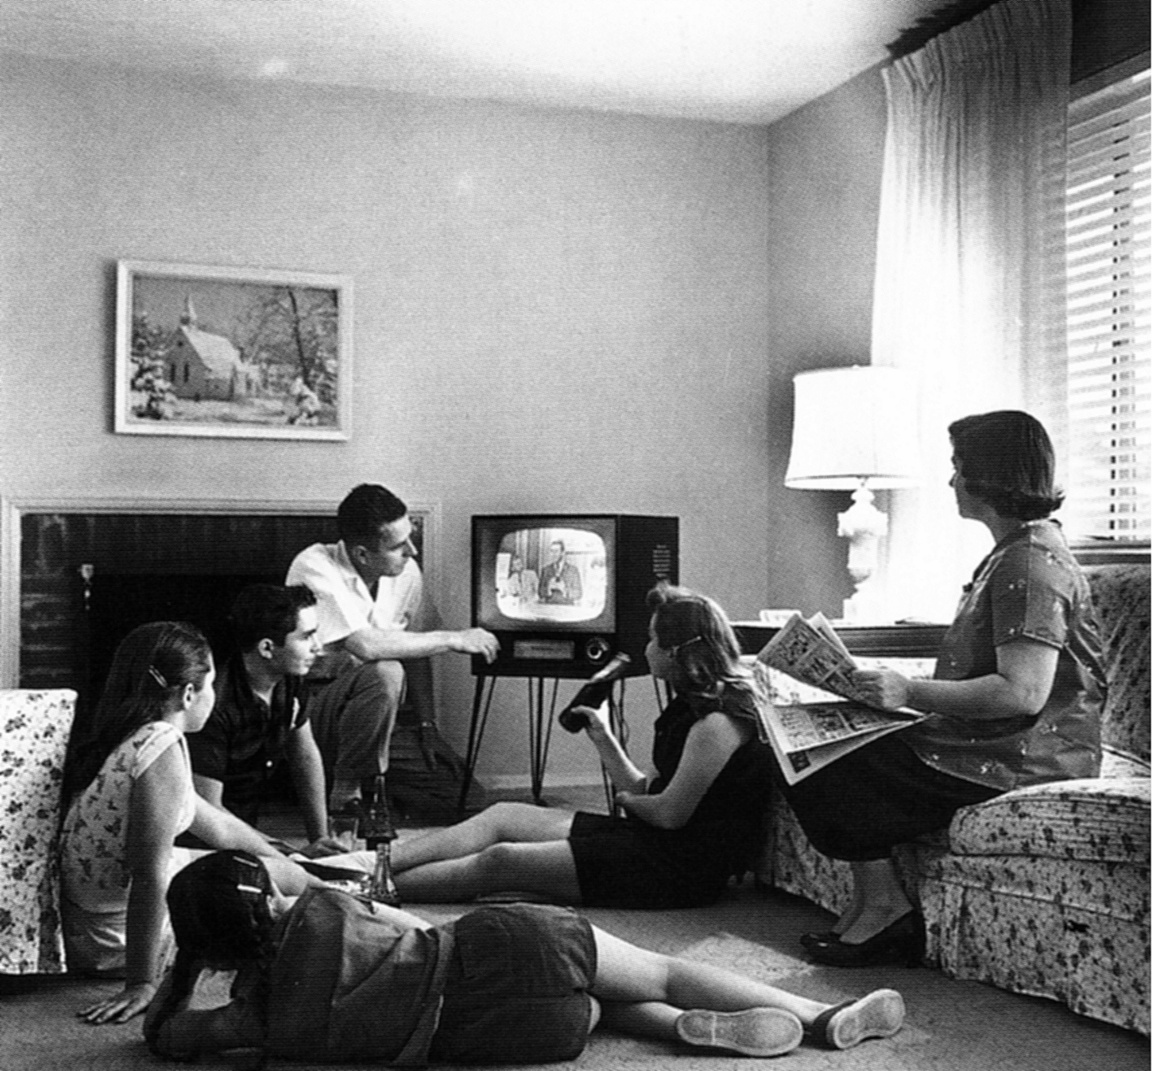
\includegraphics[height=3.4cm]{images/intro/old.jpg}~~~
				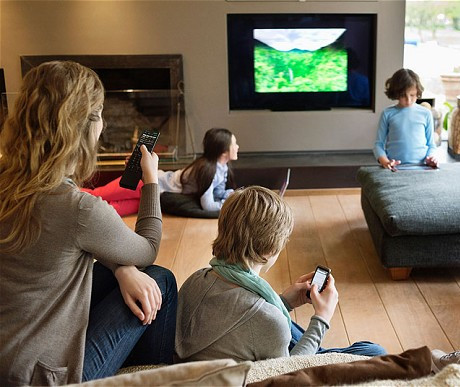
\includegraphics[height=3.4cm]{images/intro/currently.jpg}
				\caption{Les débuts de la Télévision face à son évolution}
			\end{figure}
		\end{frame}
	\begin{frame}{Problématique}
		\Large
		\begin{center}
		Quels sont les systèmes à mettre en œuvre pour offrir une expérience sociale depuis son poste de télévision ?
	\end{center}
	\end{frame}
	\begin{frame}
		\tableofcontents
	\end{frame}
	\sidetoc{yes}
	\CedricSpeak{}
	\section{La télévision interactive}
	\subsection{L'influence des personnes}
	\begin{frame}{L'influence des personnes}
		\happyUser{}
\begin{itemize}
	\item Influence des téléspectateurs
		\begin{itemize}
			\item Sur le déroulement d'une émission en directe
			\item Sur le programme/narration
				\begin{itemize}
					\item Le web (Forums, Site web dédié)
					\item Le monde réel : << The truth about Marika >>
				\end{itemize}
		\end{itemize}
\end{itemize}
	\end{frame}
	\begin{frame}{L'influence des personnes}
		\happyUser{}
		\begin{itemize}
	\item Communauté, réseaux sociaux
		\begin{itemize}
			\item Sur le site internet de l'émission
			\item Sur la page Facebook de la chaîne/émission
			\item \texttt{\#monEmission} sur Twitter
			\item Messages dans les bandeaux de l'émission
		\end{itemize}
		\begin{figure}[H]
			\hspace{-25px}
			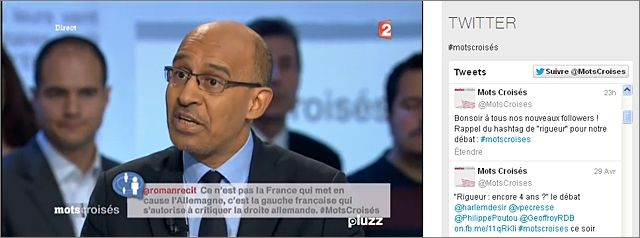
\includegraphics[height=3.5cm]{images/motscroises.jpg}
			\caption{Mots croisés sur France 2 et Twitter}
		\end{figure}
\end{itemize}
	\end{frame}
	\subsection{La communication}
	\begin{frame}{La communication}
		\only<1>{
		\happyUser{}
		}
		\only<2>{
		\unhappyUser{}
		}
\begin{itemize}
		\uncover<1->{
		\vspace{3px}
	\item Chat textuel
		\begin{itemize}
			\item Liste d'amis
			\item Éventuellement autre écran
		\end{itemize}
		\vfill
		}
		\uncover<2->{
	\item Chat vocal
		\begin{itemize}
			\item Difficile à utiliser \\
				$\Rightarrow$ Concentration\\
				$\Rightarrow$ Bruit de la TV
		\end{itemize}
		}

		\begin{figure}[H]
			\centering
			\only<1>{
			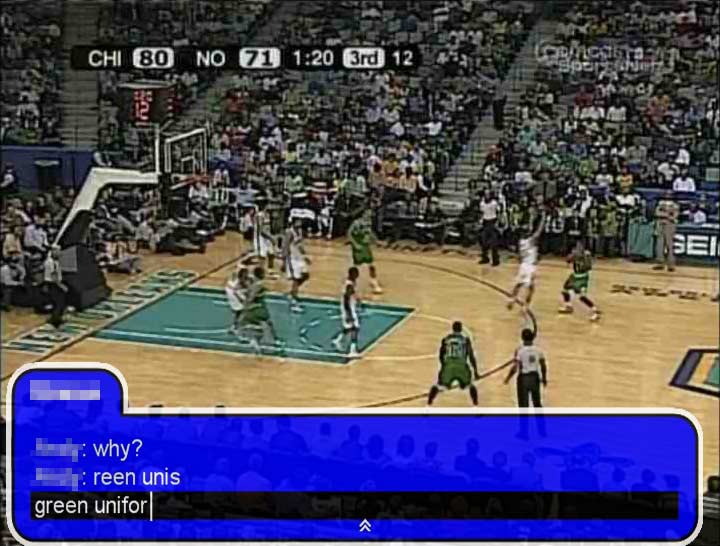
\includegraphics[height=3.7cm]{images/chats/text.png}
			\caption{
			\scriptsize
			Exemple de chat textuel\newline
			\tiny
			© Elaine M. \bsc{Huang}, Gunnar \bsc{Harboe}, Joe \bsc{Tullio},
			Ashley \bsc{Novak}, Noel \bsc{Massey}, Crysta J. \bsc{Metcalf},
			Guy \bsc{Romano}\newline
			\textit{A Field Study of Communication Choices and
			Practices Of Social Television Comes Home}
			}
			}
			\only<2>{
			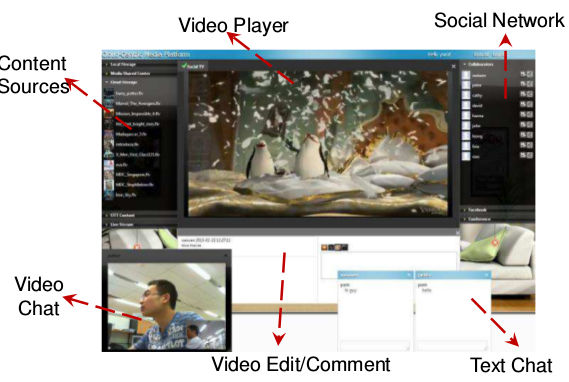
\includegraphics[height=4cm]{images/chats/textandvideo.png}
			\caption{
			\scriptsize
			Exemple d'interface avec chats\newline
			\tiny
			©Yichao \bsc{Jin}, Tian \bsc{Xie}, Yonggang \bsc{Wen}, Haiyong
			\bsc{Xie}\newline
			\textit{
			Multi-Screen Cloud Social TV:
			Transforming TV Experience into 21st Century
			}
			}
			}
		\end{figure}
		\vfill
\end{itemize}
	\end{frame}
	\AntoineSpeak{}
	\subsection{Le partage}
	\begin{frame}{Le partage : aussi sociale que Facebook ?}
		\only<1,2>{
		\happyUser{}
		}
	\begin{itemize}
			\uncover<1->{
		\item Outils de communication
			\begin{itemize}
				\item Chat, message personnel, statut
			\end{itemize}
			\vfill
			}
			\uncover<2->{
		\item Jeux interactifs
			\begin{itemize}
				\item Score, partage du score, classement
			\end{itemize}
			\vfill
			\begin{figure}[H]
	\hspace{-20px}
				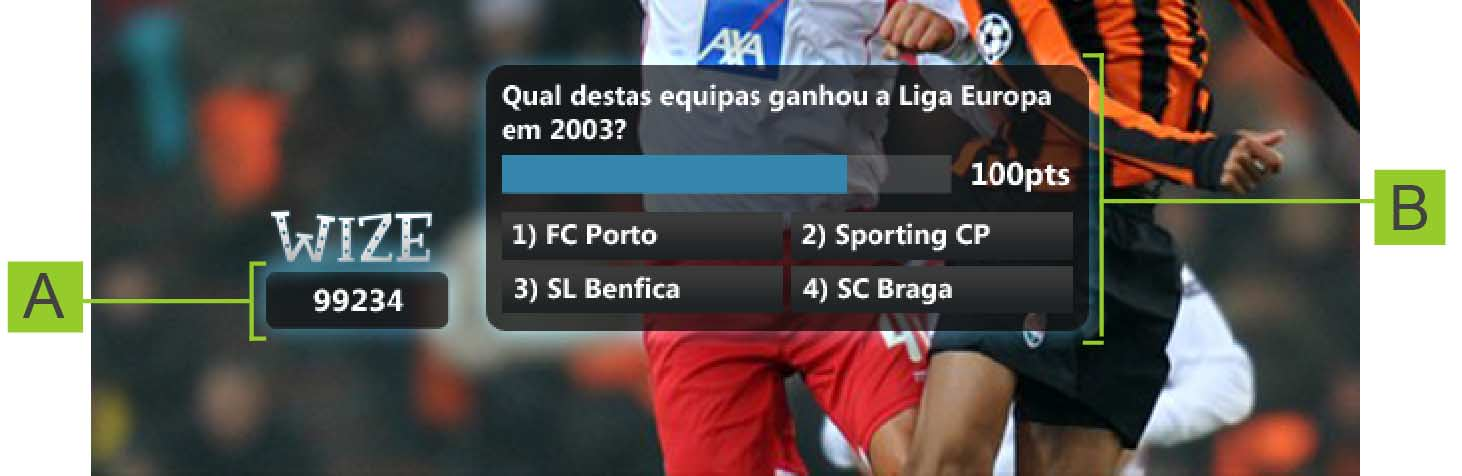
\includegraphics[height=3.0cm]{images/wize/1.png}
				\caption{Exemple du jeu interactif Wize\newline
				\tiny{
				© \bsc{Almeida}, J. \bsc{Abreu}, A. \bsc{Pinho}, D. \bsc{Costa}\newline  \textit{Engaging Viewers through Social TV
				Games}.\newline~\newline
				A : Nombres de points acquis\newline
				B : Fenêtre principale contenant la question
				}
				}
			\end{figure}
			}
			\uncover<3->{
		\item Proposition de contenu en fonction de différents critères
			\vfill
			}
	\end{itemize}
\end{frame}
\TsooSpeak{}
	\section{La télévision sur multi-écrans}
	\subsection{L'utilisation de la télévision multi-écrans}
	\begin{frame}{L'utilisation de la télévision multi-écrans}
		\happyUser{}
		\vfill
		\vfill
		\vfill
		\vfill
		\begin{exampleblock}{Avantages}
			\begin{itemize}
					\uncover<1->{
				\item Ne perturbe pas le visionnage sur la TV
					}
					\uncover<2->{
				\item Accès aux informations
					}
					\uncover<3->{
				\item Se prête bien au social
					}
					\uncover<4->{
				\item Distinction du côté social et du côté spectateur
					}
			\end{itemize}
		\end{exampleblock}
					\uncover<5->{
		\begin{alertblock}{Inconvénients}
			\begin{itemize}
				\item Attention requise
					\uncover<6->{
				\item Problème de gestion des appels sur les téléphones
					}
					\uncover<7->{
				\item Peu naturel
					}
			\end{itemize}
		\end{alertblock}
					}
	\end{frame}
	\subsection{Les écrans externes}
	\begin{frame}{Les écrans externes}
		\happyUser{}
\begin{itemize}
	\item Répartition de contenu sur plusieurs écrans
		\begin{itemize}
			\item Télévision
			\item Smartphones 
			\item Ordinateurs et tablettes
		\end{itemize}
\end{itemize}
\begin{figure}[H]
	\centering
	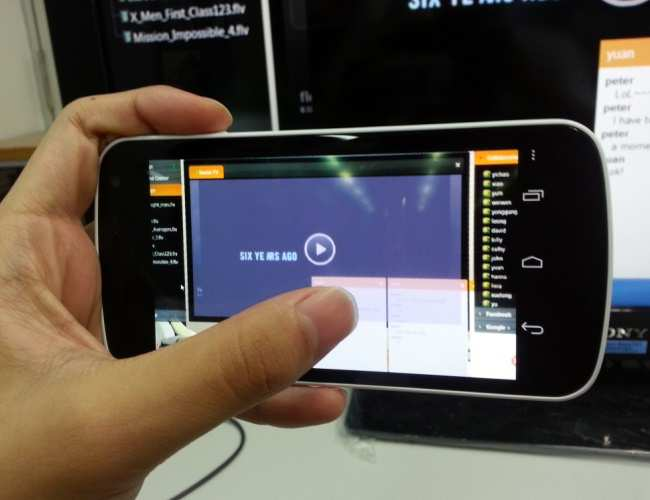
\includegraphics[height=3cm]{images/externalsScreens/1.png}~~
	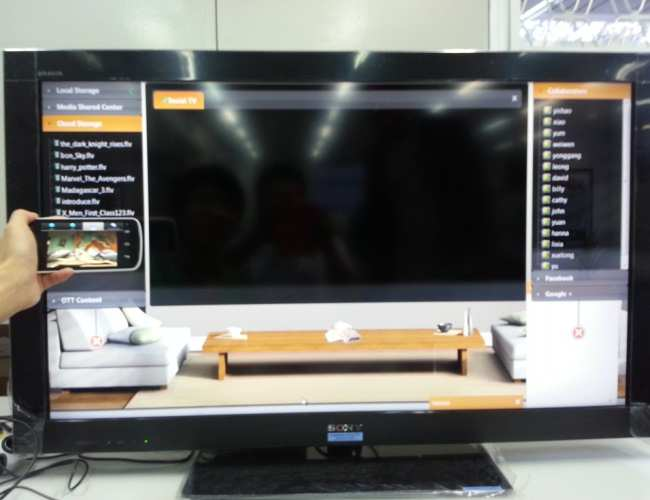
\includegraphics[height=3cm]{images/externalsScreens/2.png}

	\caption{Exemples d'écrans externes\newline
	\tiny
	© Yichao \bsc{Jin}, Tian \bsc{Xie}, Yonggang \bsc{Wen}, Haiyong \bsc{Xie}\newline
	\textit{ Multi-Screen Cloud Social TV: Transforming TV Experience into 21st Century }
	}
\end{figure}
	\end{frame}
\FlorentSpeak{}
	\section{Les systèmes et services TV}
	\subsection{Les box et périphériques}
	\begin{frame}{Les box et périphériques}
		\only<2->{
		\happyUser{}
		}
		\begin{itemize}
			\item Système $\rightarrow$ Services
		\pause
			\item Lien entre Box et autres périphériques
		\pause
			\item Périphériques externes
				\begin{itemize}
					\item Tablettes / Smartphones / PC
					\item Périphériques spécifiques
				\end{itemize}
		\end{itemize}
						\begin{figure}[H]
							\centering
							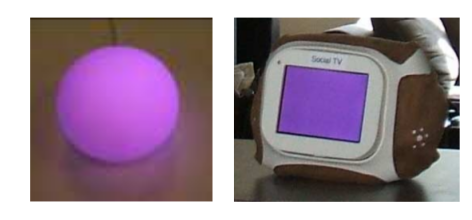
\includegraphics[width=6cm]{images/otherDevice.png}
							\caption{Exemple de périphérique
							spécifique\newline
							\tiny © Gunnar \bsc{Harboe}, Crysta J.  \bsc{Metcalf}, Frank \bsc{Bentley}, Joe \bsc{Tullio}, Noel \bsc{Massey}, Guy
							\bsc{Romano}\newline
							\textit{Ambient Social TV: Drawing People into a Shared Experience}
							}
						\end{figure}
	\end{frame}
	\subsection{Le Cloud computing}
	\begin{frame}{Le Cloud computing}
		\only<1->{
		\happyAndUnhappyUser{}
		}
		\begin{itemize}
				\uncover<1-> {
				\vspace{5px}
			\item Synchronisation
				\begin{figure}[H]
					\centering
					}
					\only<1> {
					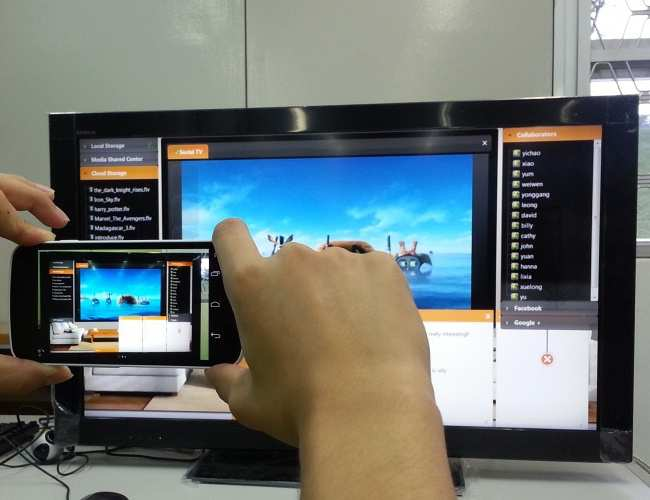
\includegraphics[height=3cm]{images/sync.png}
					}
					\only<2-> {
					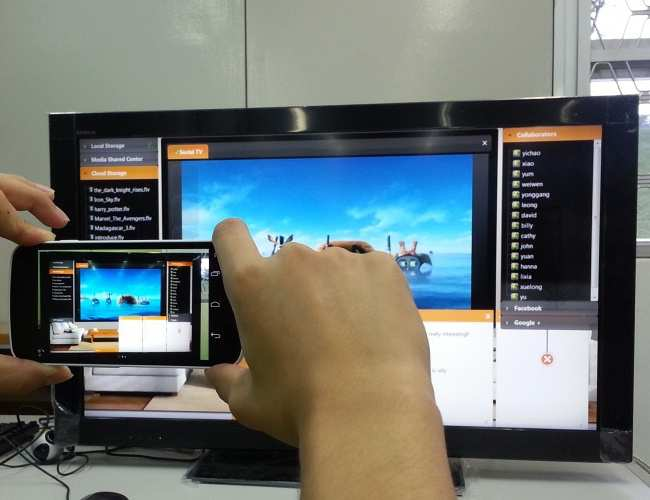
\includegraphics[height=2.0cm]{images/sync.png}
					}
					\uncover<1->{
					\caption{
					\scriptsize
					Exemple de Synchronisation\newline
					\tiny
					© Yichao \bsc{Jin}, Tian \bsc{Xie}, Yonggang \bsc{Wen}, Haiyong \bsc{Xie}\newline
					\textit{ Multi-Screen Cloud Social TV: Transforming TV Experience into 21st Century }
					}
				\end{figure}
				}
				\uncover<2->{
			\item Mise en place d'API
				\begin{figure}[H]
					\vspace{-5px}
					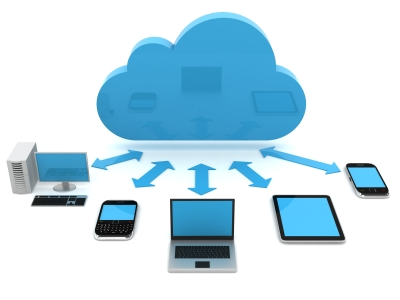
\includegraphics[height=3.1cm]{images/api.jpg}
					\vspace{-12px}
					\caption{\scriptsize Diffusion des services sur multi-écrans au moyen d'une API}
				\end{figure}
				}
		\end{itemize}
	\end{frame}
	\begin{frame}{Le Cloud computing}
		\uncover<1->{
		\footnotesize {
		\begin{exampleblock}{Avantages}
			\begin{itemize}
				\item IHM identique sur chaque périphériques connectés
				\item Passage d'un écran à un autre sans << perte d'informations >>
				\item Poursuivre le visonnage hors de chez soi en se connectant au cloud
			\end{itemize}
		\end{exampleblock}
				\vfill
				\begin{alertblock}{Inconvénient}
		\begin{itemize}
			\item Pas de distinction entre partie TV et partie Sociale
		\end{itemize}
		\end{alertblock}
		}
		}
	\end{frame}

	\AntoineSpeak{}
	\section*{}
	\hspace{-25px}
	\begin{frame}{\hspace{10px}Tableau de synthèse}
		\vspace{-5px}
		\begin{table}[H]
		\tiny
		\begin{tabular}{|p{1.4cm}|p{1.45cm}|p{0.7cm}|p{0.6cm}|p{0.6cm}|p{0.25cm}|p{1.1cm}|p{0.6cm}|}
			\hline
			&\textbf{Influence des personnes} &\textbf{Commu\-nication} &\textbf{Partage} &\textbf{Multi-écrans} &\textbf{Box} &\textbf{Périphérique} &\textbf{Cloud}\\
			\hline
			\begin{minipage}{1.4cm}
				\vspace{0.5px}
				\textbf{Chat textuel}\newline
			\vspace{-12px}
			\begin{flushleft}
			\fontsize{4.0}{4}\selectfont 
			J. Hess, B. Ley, C. Ogonowski, L. Wan, V. Wulf,E. M. Huang, G. Harboe, J. Tullio, A. Novak, N. Massey, C. J.
			Metcalf, G. Romano
		\end{flushleft}
			\end{minipage}	
			\vspace{2px}
			& \texttt{N/A} &\cmark&\cmark&\cmark&\cmark&\cmark&\cmark\\
			\hline
			\begin{minipage}{1.4cm}
				\vspace{0.5px}
				\textbf{Chat vocal} \newline
			\vspace{-12px}
			\begin{flushleft}
			\fontsize{4}{4}\selectfont
			E. M. Huang, G. Harboe, J. Tullio, A. Novak, N. Massey, C. J. Metcalf, G. Romano
		\end{flushleft}
		\end{minipage}
			\vspace{2px}
		& \texttt{N/A} &\xmark&\cmark&\xmark&\cmark&\xmark & \cmark \\
			\hline
			\begin{minipage}{1.4cm}
				\vspace{0.5px}
				\textbf{Chat vidéo}\newline
			\vspace{-12px}
			\begin{flushleft}
			\fontsize{4}{4}\selectfont
			D. Geerts, X. Li, T. Xie, and Y. Wen
		\end{flushleft}
			\end{minipage}
			\vspace{2px}
			& \texttt{N/A}&\xmark&\cmark&\xmark&\cmark&\xmark& \cmark\\
			\hline
			\begin{minipage}{1.4cm}
				\vspace{0.5px}
				\textbf{Réseau social}\newline
			\vspace{-12px}
			\begin{flushleft}
			\fontsize{4}{4}\selectfont
			T. Horozov, N. Narasimhan, J. Wickramasuriya, V. Vasudevan, A. S. Shirazi, M. Rohs, R. Schleicher, S. Kratz,
			A. Müller, A. Schmidt, M. Doughty, D. Rowland, S. Lawson
		\end{flushleft}
			\end{minipage}
			\vspace{2px}
			&\cmark&\cmark&\cmark&\cmark&\cmark&\cmark& \cmark \\
			\hline
			\begin{minipage}{1.4cm}
				\vspace{0.5px}
				\textbf{Jeu}\newline
			\vspace{-12px}
			\begin{flushleft}
			\fontsize{4}{4}\selectfont
			P. Almeida, J. Ferraz, A. Pinho, D. Costa
		\end{flushleft}
			\end{minipage}
			\vspace{2px}
			&\xmark& \texttt{N/A} &\cmark&\cmark&\cmark&\xmark& \cmark\\
			\hline
		\end{tabular}
		\caption{Synthèse des systèmes de télévision sociale\footnotemark[1]}
	\end{table}
	\footnotetext[1]{\vspace{2px}\tiny Pour plus de détails, reportez vous à notre état de l'art sur les télévisions sociales}
	\end{frame}
	\begin{frame}{Conclusion}
		\begin{itemize}
			\item TV $\rightarrow$ Sociale
				\pause
			\item Interactive
				\pause
			\item TV sur plusieurs écrans\ldots
				\pause
			\item \ldots et différents systèmes
		\end{itemize}
		\begin{figure}[H]
			\centering
			\vspace{-17px}
			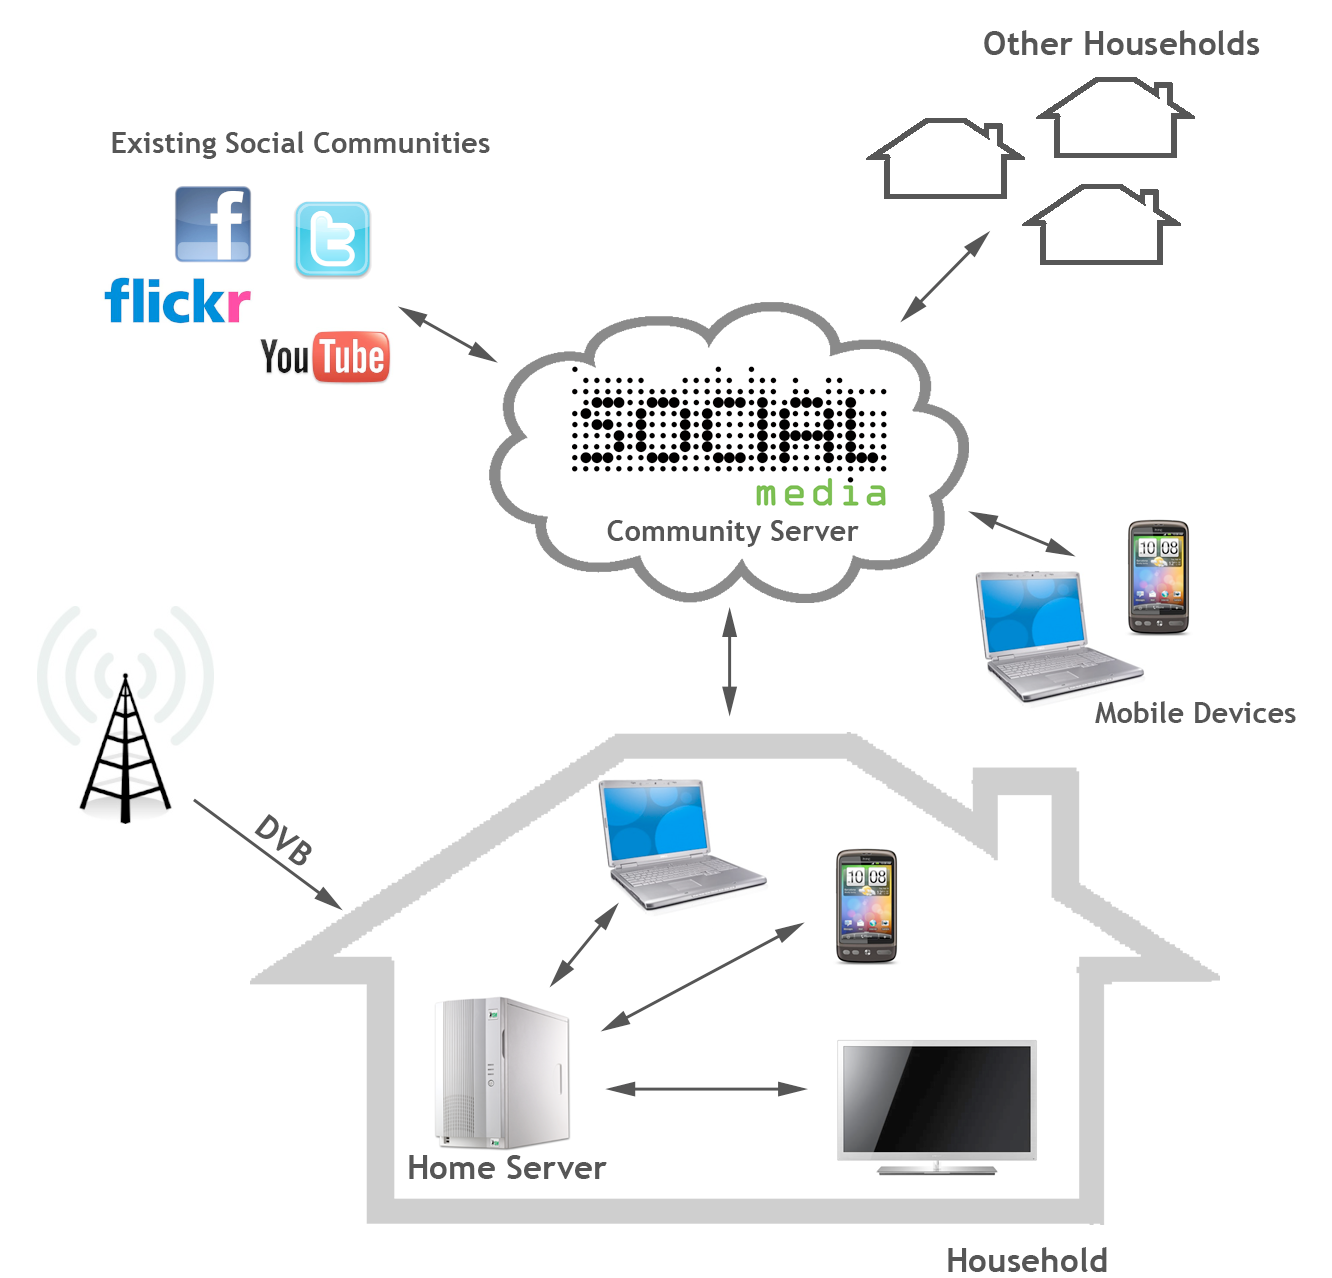
\includegraphics[width=5.4cm]{images/conclu.png}
			\scriptsize{
			\caption{SocialMediaFramework\newline 
			\tiny © Jan \bsc{Hess}, Benedikt \bsc{Ley}, Corinna \bsc{Ogonowski}, Lin \bsc{Wan}, Volker \bsc{Wulf}\newline
			\textit{Jumping between Devices and Services: Towards an Integrated Concept for Social TV}
			}
		}
		\end{figure}
	\end{frame}
	\sidetoc{no}
	\NooneSpeak{}
	\begin{frame}{Avez-vous des questions ?}
		\begin{figure}[H]
			\centering
			
\includegraphics[width=5cm]{questions.png}
		\end{figure}
	\end{frame}
	\begin{frame}
		\titlepage
	\end{frame}

\end{document}
